\documentclass[12pt, a4paper]{article}

% ── Packages ──
\usepackage[utf8]{inputenc}
\usepackage[T1]{fontenc}
\usepackage{lmodern}
\usepackage[margin=1in]{geometry}
\usepackage{graphicx}
\usepackage{xcolor}
\usepackage{listings}
\usepackage{hyperref}
\usepackage{tikz}
\usepackage{enumitem}
\usepackage{tcolorbox}
\usepackage{fancyhdr}
\usepackage{titlesec}
\usepackage{booktabs}
\usepackage{longtable}
\usepackage{float}
\usepackage{amsmath}
\usepackage{forest}

\usetikzlibrary{shapes.geometric, arrows.meta, positioning, fit, calc, backgrounds}
\tcbuselibrary{skins, breakable}

% ── Colors ──
\definecolor{zygotePrimary}{HTML}{6C5CE7}
\definecolor{zygoteSecondary}{HTML}{00B894}
\definecolor{zygoteAccent}{HTML}{FD79A8}
\definecolor{zygoteDark}{HTML}{2D3436}
\definecolor{zygoteLight}{HTML}{DFE6E9}
\definecolor{codeBg}{HTML}{F8F9FA}
\definecolor{codeFrame}{HTML}{DEE2E6}
\definecolor{nodeBlue}{HTML}{74B9FF}
\definecolor{nodePurple}{HTML}{A29BFE}
\definecolor{nodeGreen}{HTML}{55EFC4}
\definecolor{nodeOrange}{HTML}{FDCB6E}
\definecolor{nodeRed}{HTML}{FF7675}
\definecolor{linkColor}{HTML}{0984E3}

% ── Hyperref setup ──
\hypersetup{
    colorlinks=true,
    linkcolor=linkColor,
    urlcolor=linkColor,
    citecolor=linkColor,
    pdftitle={Zygote Architecture Guide},
    pdfauthor={Zygote AI},
}

% ── Code listing style ──
\lstdefinestyle{tsStyle}{
    language=Java,
    basicstyle=\ttfamily\small,
    backgroundcolor=\color{codeBg},
    frame=single,
    rulecolor=\color{codeFrame},
    keywordstyle=\color{zygotePrimary}\bfseries,
    stringstyle=\color{zygoteSecondary},
    commentstyle=\color{gray}\itshape,
    numbers=left,
    numberstyle=\tiny\color{gray},
    numbersep=8pt,
    breaklines=true,
    breakatwhitespace=true,
    tabsize=2,
    showstringspaces=false,
    xleftmargin=15pt,
    framexleftmargin=15pt,
    morekeywords={interface, type, export, const, let, async, await, import, from, extends, implements, readonly, string, number, boolean, null, undefined, Record, Promise, void},
    literate={=>}{{\textcolor{zygoteAccent}{=>}}}{2}
             {|}{{\textcolor{zygoteAccent}{|}}}{1},
}
\lstset{style=tsStyle}

% ── Custom boxes ──
\newtcolorbox{conceptbox}[1]{
    colback=zygotePrimary!5,
    colframe=zygotePrimary!80,
    fonttitle=\bfseries\color{white},
    title=#1,
    rounded corners,
    arc=3mm,
    boxrule=1pt,
    breakable,
}

\newtcolorbox{keypoint}{
    colback=zygoteSecondary!8,
    colframe=zygoteSecondary!60,
    fontupper=\small,
    rounded corners,
    arc=2mm,
    boxrule=0.8pt,
    left=8pt,
    right=8pt,
    breakable,
}

\newtcolorbox{warningbox}{
    colback=nodeOrange!10,
    colframe=nodeOrange!80,
    fontupper=\small,
    rounded corners,
    arc=2mm,
    boxrule=0.8pt,
    left=8pt,
    right=8pt,
}

\newtcolorbox{filebox}[1]{
    colback=codeBg,
    colframe=codeFrame,
    fonttitle=\ttfamily\small\bfseries,
    title=\textcolor{zygoteDark}{#1},
    rounded corners,
    arc=2mm,
    boxrule=0.5pt,
    breakable,
}

% ── Headers ──
\pagestyle{fancy}
\fancyhf{}
\fancyhead[L]{\small\textcolor{gray}{Zygote Architecture Guide}}
\fancyhead[R]{\small\textcolor{gray}{v0.1.0}}
\fancyfoot[C]{\thepage}
\renewcommand{\headrulewidth}{0.4pt}

% ── Section styling ──
\titleformat{\section}
    {\Large\bfseries\color{zygoteDark}}
    {\thesection}{1em}{}
    [\vspace{-0.5em}\textcolor{zygotePrimary}{\rule{\textwidth}{1.5pt}}]

\titleformat{\subsection}
    {\large\bfseries\color{zygoteDark}}
    {\thesubsection}{1em}{}

\titleformat{\subsubsection}
    {\normalsize\bfseries\color{zygotePrimary}}
    {\thesubsubsection}{1em}{}

% ══════════════════════════════════════════════════════════════
\begin{document}

% ── Title Page ──
\begin{titlepage}
\centering
\vspace*{2cm}

{\Huge\bfseries\textcolor{zygoteDark}{Zygote}}\\[0.5cm]
{\Large\textcolor{zygotePrimary}{Architecture \& Codebase Guide}}\\[2cm]

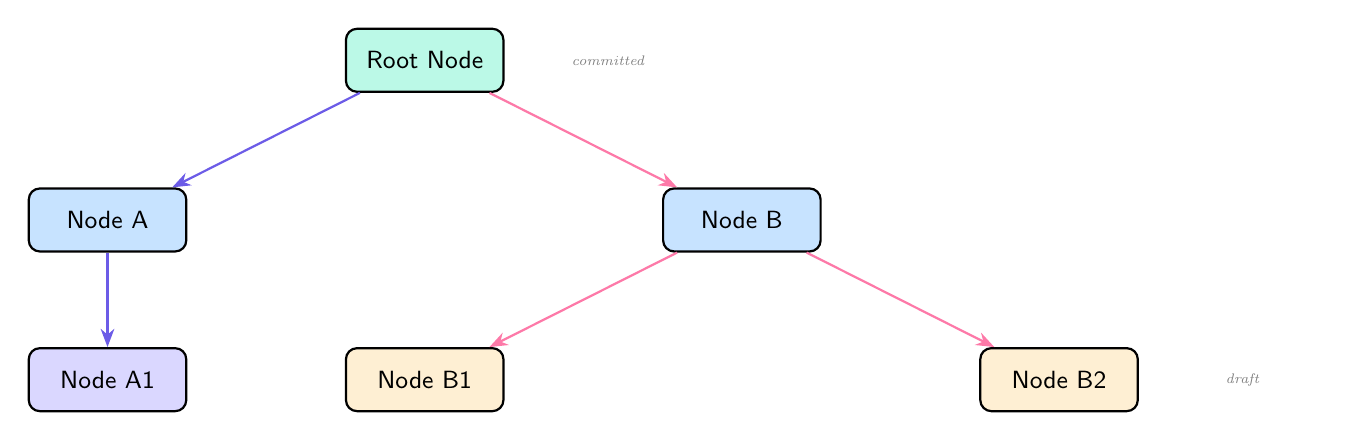
\begin{tikzpicture}[
    node distance=1.2cm and 2cm,
    every node/.style={
        draw, rounded corners=4pt, minimum width=2cm, minimum height=0.8cm,
        font=\small\sffamily, thick
    }
]
    \node[fill=nodeGreen!40] (root) {Root Node};
    \node[fill=nodeBlue!40, below left=of root] (a) {Node A};
    \node[fill=nodeBlue!40, below right=of root] (b) {Node B};
    \node[fill=nodePurple!40, below=of a] (a1) {Node A1};
    \node[fill=nodeOrange!30, below left=of b] (b1) {Node B1};
    \node[fill=nodeOrange!30, below right=of b] (b2) {Node B2};

    \draw[-Stealth, thick, zygotePrimary] (root) -- (a);
    \draw[-Stealth, thick, zygoteAccent] (root) -- (b);
    \draw[-Stealth, thick, zygotePrimary] (a) -- (a1);
    \draw[-Stealth, thick, zygoteAccent] (b) -- (b1);
    \draw[-Stealth, thick, zygoteAccent] (b) -- (b2);

    \node[draw=none, right=0.3cm of root, font=\tiny\itshape\color{gray}] {committed};
    \node[draw=none, right=0.3cm of b2, font=\tiny\itshape\color{gray}] {draft};
\end{tikzpicture}

\vspace{2cm}

{\large A complete guide to understanding every file, data structure,\\
and data flow in the Zygote VS Code extension.}\\[1cm]

\textcolor{gray}{Version 0.1.0 \quad|\quad \today}\\[0.5cm]
\textcolor{gray}{Total codebase: $\sim$4,900 lines of TypeScript}

\vfill
{\small\textcolor{gray}{This document is designed to be read section by section.\\
Each section is self-contained and builds on the previous ones.}}
\end{titlepage}

% ── Table of Contents ──
\tableofcontents
\newpage

% ══════════════════════════════════════════════════════════════
\section{What Is Zygote?}
% ══════════════════════════════════════════════════════════════

\begin{conceptbox}{The One-Sentence Summary}
Zygote is a VS Code extension that replaces linear AI chat with a \textbf{tree of work nodes}, where each node is a committed unit of work with its own file snapshot, and you can fork branches to try alternatives.
\end{conceptbox}

\subsection{The Problem Zygote Solves}

Traditional AI coding assistants (ChatGPT, Copilot Chat, Claude chat) work in a \textbf{linear conversation}. You ask something, the AI responds, and you continue forward. If the AI goes in a wrong direction, you either:

\begin{enumerate}[label=(\alph*)]
    \item Undo manually and re-prompt (losing the context of what was tried)
    \item Start a new chat (losing all prior context)
    \item Keep going and hope to fix it later
\end{enumerate}

None of these are good. Zygote solves this by making the conversation a \textbf{tree}, not a line.

\subsection{The Mental Model}

Think of Zygote like \textbf{Git for AI conversations}:

\begin{itemize}[leftmargin=2cm]
    \item[\textbf{Node}] = A commit. Contains a prompt, the AI's response, and a snapshot of all files at that point.
    \item[\textbf{Branch}] = A named line of work. Has a head node (the tip).
    \item[\textbf{Fork}] = Creating a new branch from any committed node. Files revert to that node's state.
    \item[\textbf{Switch}] = Changing which branch is active. Files automatically restore.
\end{itemize}

\begin{keypoint}
\textbf{Key insight:} Every committed node stores the exact state of every file in your workspace at that moment. When you switch branches or fork, Zygote restores those files. You can freely explore alternatives without fear of losing work.
\end{keypoint}

\subsection{Technology Stack}

\begin{table}[H]
\centering
\begin{tabular}{@{}lll@{}}
\toprule
\textbf{Layer} & \textbf{Technology} & \textbf{Purpose} \\
\midrule
Extension Host & Node.js, TypeScript & Business logic, state, agent \\
VS Code API & \texttt{vscode} module & Extension lifecycle, webview, file I/O \\
Webview UI & React 19, Vite 6 & UI rendering in webview sandbox \\
Markdown & react-markdown, rehype-highlight & Render agent output \\
Agent (SDK) & @anthropic-ai/sdk v0.98+ & Claude API calls \\
Agent (CLI) & claude-agent-sdk v0.3+ & CLI backend fallback \\
Build & TypeScript 5.8, Vite 6 & Compilation and bundling \\
\bottomrule
\end{tabular}
\end{table}

\newpage

% ══════════════════════════════════════════════════════════════
\section{Project Directory Structure}
% ══════════════════════════════════════════════════════════════

This section maps every directory and file in the project. Use it as a reference when navigating the codebase.

\subsection{Top-Level Layout}

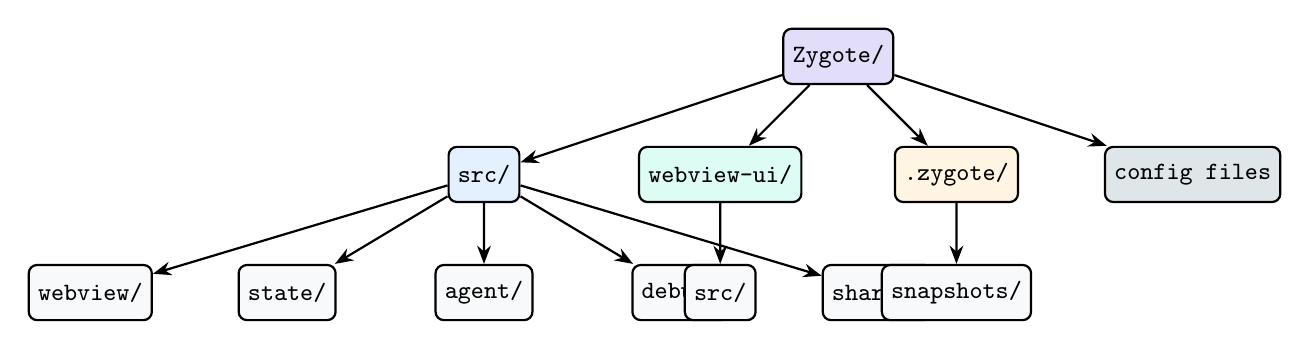
\begin{tikzpicture}[
    grow=down,
    level distance=1.5cm,
    sibling distance=3.5cm,
    every node/.style={
        draw, rounded corners=3pt, minimum height=0.7cm,
        font=\small\ttfamily, thick, fill=codeBg
    },
    edge from parent/.style={draw, thick, -Stealth},
    level 1/.style={sibling distance=3cm},
    level 2/.style={sibling distance=2.5cm},
]
    \node[fill=zygotePrimary!20] {Zygote/}
        child { node[fill=nodeBlue!20] {src/}
            child { node {webview/} }
            child { node {state/} }
            child { node {agent/} }
            child { node {debug/} }
            child { node {shared/} }
        }
        child { node[fill=nodeGreen!20] {webview-ui/}
            child { node {src/} }
        }
        child { node[fill=nodeOrange!20] {.zygote/}
            child { node {snapshots/} }
        }
        child { node[fill=zygoteLight] {config files} };
\end{tikzpicture}

\subsection{Complete File Tree}

\begin{filebox}{Zygote/ --- Root Directory}
\begin{tabular}{@{}p{6.5cm}p{7.5cm}@{}}
\texttt{package.json} & VS Code extension manifest, dependencies, scripts \\
\texttt{tsconfig.json} & TypeScript config (ES2022, strict, Node16 modules) \\
\texttt{SPEC.md} & Product specification (693 lines) \\
\texttt{PLAN.md} & Development plan and checklist \\
\texttt{zygote-strategic-roadmap.md} & 18--24 month strategic roadmap \\
\end{tabular}
\end{filebox}

\begin{filebox}{src/ --- Extension Host Source (Node.js)}
\begin{tabular}{@{}p{6.5cm}p{7.5cm}@{}}
\texttt{extension.ts} \hfill \textit{68 lines} & Entry point. Registers VS Code commands. \\
\texttt{webview/ZygotePanel.ts} \hfill \textit{$\sim$900 lines} & The brain. Message routing, state orchestration. \\
\texttt{webview/html.ts} & HTML scaffold for webview with CSP headers. \\
\texttt{state/tree.ts} \hfill \textit{$\sim$450 lines} & Pure state operations on the tree. \\
\texttt{state/persistence.ts} \hfill \textit{90 lines} & Load/save \texttt{tree.json} to disk. \\
\texttt{state/snapshots.ts} \hfill \textit{107 lines} & Content-addressable file storage (SHA-256). \\
\texttt{agent/claude.ts} \hfill \textit{84 lines} & Anthropic API client singleton. \\
\texttt{agent/tools.ts} \hfill \textit{192 lines} & 4 tool definitions + executors. \\
\texttt{agent/runner.ts} \hfill \textit{$\sim$450 lines} & Agent execution loop, preview workflow. \\
\texttt{debug/logger.ts} \hfill \textit{317 lines} & Debug logging + tree dumps. \\
\texttt{shared/types.ts} \hfill \textit{84 lines} & Shared TypeScript type definitions. \\
\end{tabular}
\end{filebox}

\begin{filebox}{webview-ui/src/ --- React UI (Webview Sandbox)}
\begin{tabular}{@{}p{6.5cm}p{7.5cm}@{}}
\texttt{main.tsx} & React bootstrap entry point. \\
\texttt{App.tsx} \hfill \textit{$\sim$470 lines} & Main app component, layout, state. \\
\texttt{vscode-api.ts} & Wrapper around \texttt{acquireVsCodeApi()}. \\
\texttt{components/TreeCanvas.tsx} & Interactive tree visualization. \\
\texttt{components/NodeDetail.tsx} & Right panel: selected node details. \\
\texttt{components/NodeChat.tsx} & Chat interface within a node. \\
\texttt{components/FloatingChat.tsx} & Ephemeral quick-ask popup. \\
\texttt{components/BranchSelector.tsx} & Branch switching dropdown. \\
\texttt{components/MarkdownRenderer.tsx} & Markdown rendering with syntax highlighting. \\
\texttt{components/ThinkingBlock.tsx} & Expandable thinking blocks display. \\
\texttt{components/Tree.tsx} & Tree display (may be superseded). \\
\end{tabular}
\end{filebox}

\begin{filebox}{.zygote/ --- Runtime Data (per workspace, gitignored)}
\begin{tabular}{@{}p{6.5cm}p{7.5cm}@{}}
\texttt{tree.json} & Full tree state (nodes, branches, snapshots). \\
\texttt{snapshots/<sha256>} & Content-addressable file blobs. \\
\end{tabular}
\end{filebox}

\newpage

% ══════════════════════════════════════════════════════════════
\section{The Three-Layer Architecture}
% ══════════════════════════════════════════════════════════════

Zygote has three distinct layers. Understanding how they communicate is the key to understanding the whole system.

\subsection{Architecture Diagram}

\begin{center}
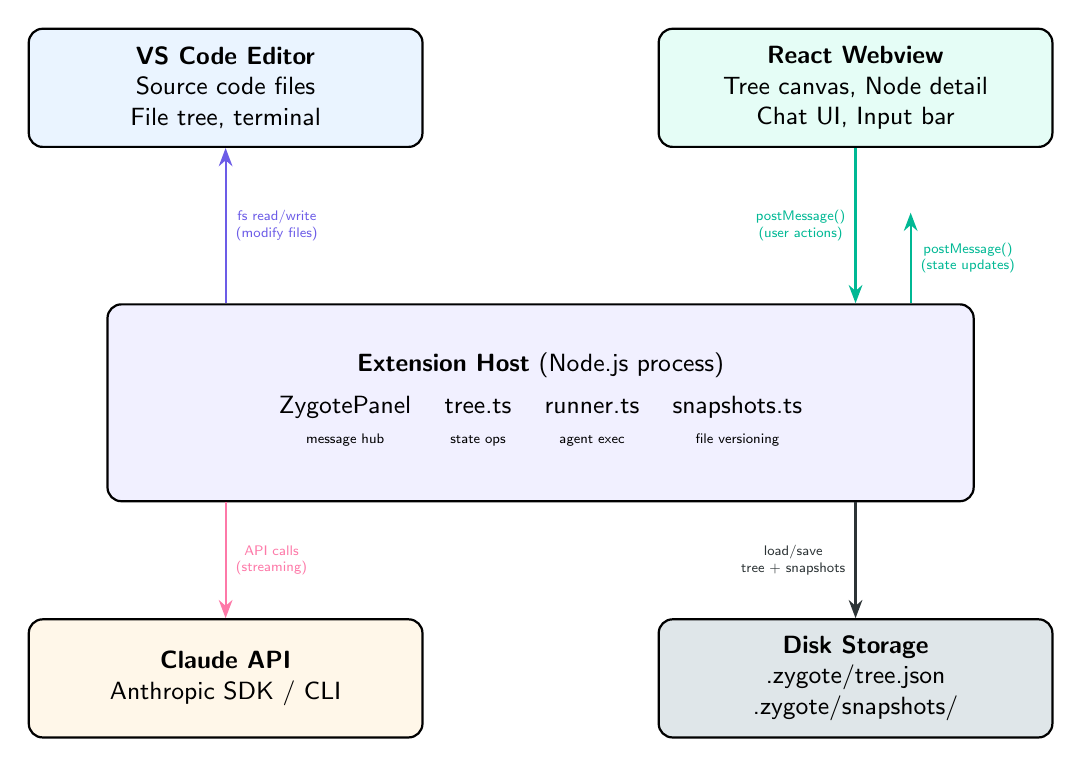
\begin{tikzpicture}[
    box/.style={draw, rounded corners=5pt, thick, minimum width=5cm, minimum height=1.5cm, align=center, font=\small\sffamily},
    arrow/.style={-Stealth, thick},
    label/.style={font=\tiny\sffamily\color{gray}, align=center},
]
    % Layer 1: Editor
    \node[box, fill=nodeBlue!15] (editor) at (-4, 4) {
        \textbf{VS Code Editor}\\
        Source code files\\
        File tree, terminal
    };

    % Layer 2: Webview
    \node[box, fill=nodeGreen!15] (webview) at (4, 4) {
        \textbf{React Webview}\\
        Tree canvas, Node detail\\
        Chat UI, Input bar
    };

    % Layer 3: Extension Host
    \node[box, fill=nodePurple!15, minimum width=11cm, minimum height=2.5cm] (host) at (0, 0) {
        \textbf{Extension Host} (Node.js process)\\[4pt]
        \begin{tabular}{cccc}
        ZygotePanel & tree.ts & runner.ts & snapshots.ts \\
        \tiny message hub & \tiny state ops & \tiny agent exec & \tiny file versioning
        \end{tabular}
    };

    % Layer 4: External
    \node[box, fill=nodeOrange!15, minimum width=5cm] (claude) at (-4, -3.5) {
        \textbf{Claude API}\\
        Anthropic SDK / CLI
    };

    \node[box, fill=zygoteLight, minimum width=5cm] (disk) at (4, -3.5) {
        \textbf{Disk Storage}\\
        .zygote/tree.json\\
        .zygote/snapshots/
    };

    % Arrows
    \draw[arrow, zygotePrimary] (host.north -| editor.south) -- (editor.south)
        node[label, midway, right] {fs read/write\\(modify files)};
    \draw[arrow, zygoteSecondary] (webview.south) -- (host.north -| webview.south)
        node[label, midway, left] {postMessage()\\(user actions)};
    \draw[arrow, zygoteSecondary] (host.north -| webview.south) ++(0.7,0) -- ++(0, 1.15)
        node[label, midway, right] {postMessage()\\(state updates)};
    \draw[arrow, zygoteAccent] (host.south -| claude.north) -- (claude.north)
        node[label, midway, right] {API calls\\(streaming)};
    \draw[arrow, zygoteDark] (host.south -| disk.north) -- (disk.north)
        node[label, midway, left] {load/save\\tree + snapshots};
\end{tikzpicture}
\end{center}

\subsection{Layer Responsibilities}

\begin{table}[H]
\centering
\begin{tabular}{@{}p{3cm}p{4.5cm}p{5.5cm}@{}}
\toprule
\textbf{Layer} & \textbf{Runs In} & \textbf{Responsibility} \\
\midrule
VS Code Editor & VS Code main process & Displays source code files. Agent modifies files here via \texttt{vscode.workspace.fs}. \\[6pt]
React Webview & Sandboxed iframe & UI only. Renders the tree, node details, chat. Cannot access the filesystem. \\[6pt]
Extension Host & Node.js child process & \textbf{Source of truth.} Holds the tree, runs the agent, does file I/O, persists state. \\
\bottomrule
\end{tabular}
\end{table}

\begin{warningbox}
\textbf{Critical rule:} The Extension Host is the single source of truth. The webview is a \textit{view layer only}. It receives the full tree via \texttt{treeUpdated} messages and renders it. All mutations happen in the extension host.
\end{warningbox}

\newpage

% ══════════════════════════════════════════════════════════════
\section{Core Data Model}
% ══════════════════════════════════════════════════════════════

Everything in Zygote revolves around three data structures: \textbf{ZygoteTree}, \textbf{ZygoteNode}, and \textbf{ZygoteBranch}. They are defined in \texttt{src/shared/types.ts}.

\subsection{ZygoteTree --- The Root Container}

\begin{lstlisting}
interface ZygoteTree {
  workspaceRoot: string;           // VS Code workspace path
  rootNodeIds: NodeId[];           // Top-level entry points
  nodes: Record<NodeId, ZygoteNode>; // FLAT map of all nodes
  branches: Record<BranchId, ZygoteBranch>;
  activeBranchId: BranchId;       // Currently "checked out" branch
}
\end{lstlisting}

\begin{keypoint}
\textbf{Why a flat map?} Nodes are stored in a flat \texttt{Record<NodeId, ZygoteNode>}, not nested objects. The tree structure comes from each node's \texttt{parentId} pointer. This gives O(1) lookup by ID, easy serialization to JSON, and simple traversal.
\end{keypoint}

\subsection{ZygoteNode --- The Atomic Unit of Work}

Each node represents one prompt--response cycle with its associated file state.

\begin{lstlisting}
interface ZygoteNode {
  id: NodeId;                     // UUID
  parentId: NodeId | null;        // Tree link (null = root)
  branchId: BranchId;             // Which branch owns this node
  status: NodeStatus;             // 'draft'|'previewing'|'committed'|'error'
  title: string;                  // Display label (auto-summarized)
  prompt: string;                 // User's instruction
  chat: ChatMessage[];            // Pre-execution conversation
  agentResponse?: string;         // Claude's full text output
  thinkingContent?: string;       // Extended thinking blocks
  toolCalls?: ToolCall[];         // File operations performed
  workspaceSnapshot?: {           // File state at commit time
    fileHashes: Record<string, FileHash>
  };
  tokens?: { input: number; output: number };
  error?: string;                 // Error message if status='error'
}
\end{lstlisting}

\subsection{Node Status Lifecycle}

\begin{center}
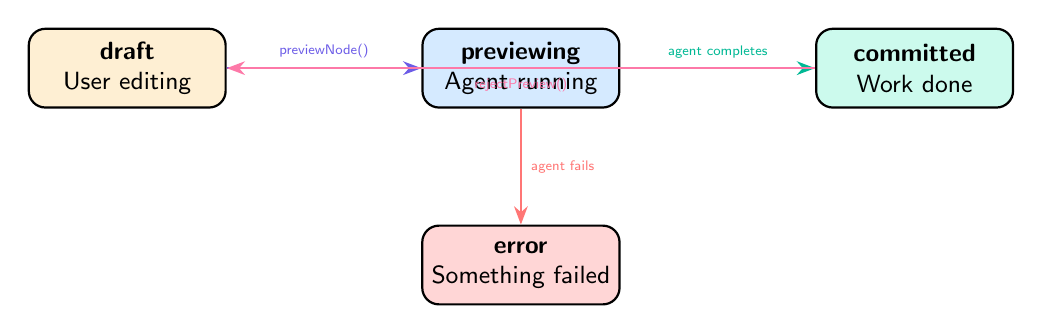
\begin{tikzpicture}[
    state/.style={draw, rounded corners=6pt, thick, minimum width=2.5cm, minimum height=1cm, align=center, font=\sffamily\small},
    arrow/.style={-Stealth, thick},
]
    \node[state, fill=nodeOrange!30] (draft) at (0, 0) {\textbf{draft}\\User editing};
    \node[state, fill=nodeBlue!30] (previewing) at (5, 0) {\textbf{previewing}\\Agent running};
    \node[state, fill=nodeGreen!30] (committed) at (10, 0) {\textbf{committed}\\Work done};
    \node[state, fill=nodeRed!30] (error) at (5, -2.5) {\textbf{error}\\Something failed};

    \draw[arrow, zygotePrimary] (draft) -- (previewing)
        node[above, midway, font=\tiny\sffamily] {previewNode()};
    \draw[arrow, zygoteSecondary] (previewing) -- (committed)
        node[above, midway, font=\tiny\sffamily] {agent completes};
    \draw[arrow, zygoteAccent] (committed) -- (draft)
        node[below, midway, font=\tiny\sffamily, sloped] {rejectPreview()};
    \draw[arrow, nodeRed] (previewing) -- (error)
        node[right, midway, font=\tiny\sffamily] {agent fails};
\end{tikzpicture}
\end{center}

\begin{itemize}
    \item \textbf{draft}: Node exists but agent hasn't run. User can edit prompt, add chat messages.
    \item \textbf{previewing}: Agent is currently executing. Workspace is locked.
    \item \textbf{committed}: Agent finished. Results (response, tool calls, file snapshot) are stored.
    \item \textbf{error}: Agent execution failed. Error message stored in node.
\end{itemize}

\subsection{ZygoteBranch --- A Named Line of Work}

\begin{lstlisting}
interface ZygoteBranch {
  id: BranchId;                   // UUID
  name: string;                   // "main", "try-middleware", etc.
  headNodeId: NodeId | null;      // Tip of this branch
  parentBranchId?: BranchId;      // Forked from which branch
  forkedAtNodeId?: NodeId;        // Forked at which node
  createdAt: number;              // Timestamp
}
\end{lstlisting}

\begin{keypoint}
\textbf{Forking is O(1).} When you fork, Zygote only creates a new branch entry pointing to the fork node. No nodes are copied. The new branch simply shares ancestor nodes with the original branch.
\end{keypoint}

\subsection{How Tree Structure Works}

\begin{center}
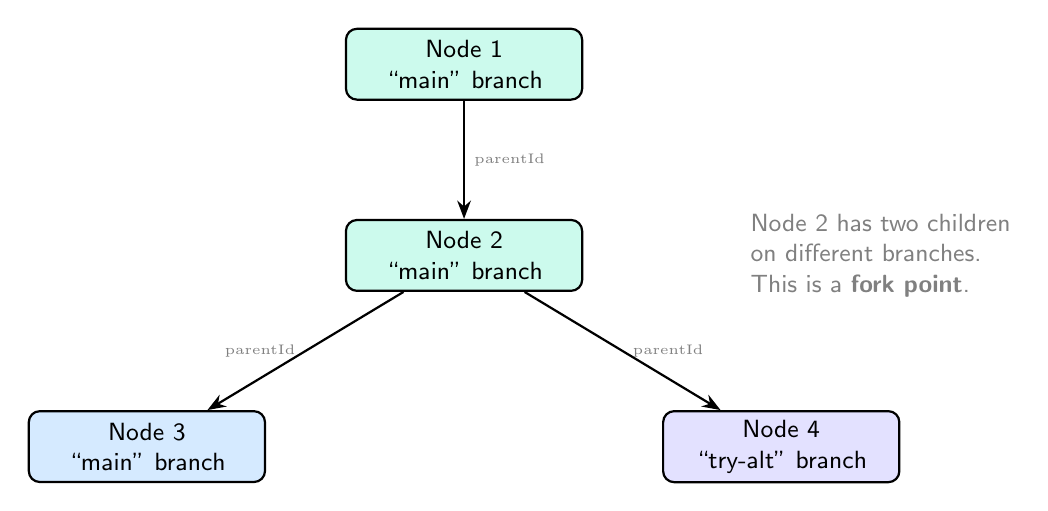
\begin{tikzpicture}[
    node distance=1.5cm,
    treenode/.style={draw, rounded corners=4pt, thick, minimum width=3cm, minimum height=0.9cm, font=\small\sffamily, align=center},
    arrow/.style={-Stealth, thick},
]
    \node[treenode, fill=nodeGreen!30] (n1) {Node 1\\``main'' branch};
    \node[treenode, fill=nodeGreen!30, below=of n1] (n2) {Node 2\\``main'' branch};
    \node[treenode, fill=nodeBlue!30, below left=1.5cm and 1cm of n2] (n3) {Node 3\\``main'' branch};
    \node[treenode, fill=nodePurple!30, below right=1.5cm and 1cm of n2] (n4) {Node 4\\``try-alt'' branch};

    \draw[arrow] (n1) -- (n2) node[midway, right, font=\tiny\color{gray}] {parentId};
    \draw[arrow] (n2) -- (n3) node[midway, left, font=\tiny\color{gray}] {parentId};
    \draw[arrow] (n2) -- (n4) node[midway, right, font=\tiny\color{gray}] {parentId};

    \node[draw=none, right=2cm of n2, font=\small\sffamily, align=left, text=gray] {
        Node 2 has two children\\
        on different branches.\\
        This is a \textbf{fork point}.
    };
\end{tikzpicture}
\end{center}

The nodes are stored flat:
\begin{lstlisting}
nodes: {
  "node-1": { id: "node-1", parentId: null,     branchId: "main-branch" },
  "node-2": { id: "node-2", parentId: "node-1", branchId: "main-branch" },
  "node-3": { id: "node-3", parentId: "node-2", branchId: "main-branch" },
  "node-4": { id: "node-4", parentId: "node-2", branchId: "try-alt" },
}
\end{lstlisting}

\newpage

% ══════════════════════════════════════════════════════════════
\section{Message Protocol}
% ══════════════════════════════════════════════════════════════

The webview and extension host communicate via \texttt{postMessage()}. Every user action and every state update flows through this channel.

\subsection{Webview $\to$ Extension (User Actions)}

\begin{longtable}{@{}p{4.5cm}p{4cm}p{5cm}@{}}
\toprule
\textbf{Message Type} & \textbf{Payload} & \textbf{What Happens} \\
\midrule
\endhead
\texttt{createNode} & parentId, prompt & Creates draft node, auto-runs preview \\
\texttt{updateNodePrompt} & nodeId, prompt & Edits draft node's prompt \\
\texttt{updateNodeTitle} & nodeId, title & Renames node \\
\texttt{appendChatMessage} & nodeId, role, content & Adds chat message to node \\
\texttt{requestChatResponse} & nodeId & Runs agent on node's chat \\
\texttt{previewNode} & nodeId & Begins preview execution \\
\texttt{rejectPreview} & nodeId & Reverts files, returns to draft \\
\texttt{switchBranch} & branchId & Switches active branch + restores files \\
\texttt{deleteNode} & nodeId & Deletes leaf draft node \\
\texttt{deleteBranch} & branchId & Cascade deletes branch + children \\
\texttt{saveAndCheckout} & fromNodeId, toNodeId & Checkpoint and restore \\
\texttt{quickAsk} & prompt & Ephemeral floating chat (not persisted) \\
\bottomrule
\end{longtable}

\subsection{Extension $\to$ Webview (State Updates)}

\begin{longtable}{@{}p{4.5cm}p{4cm}p{5cm}@{}}
\toprule
\textbf{Message Type} & \textbf{Payload} & \textbf{What It Does} \\
\midrule
\endhead
\texttt{treeUpdated} & tree (full ZygoteTree) & Full state refresh \\
\texttt{nodeOutputStream} & nodeId, delta & Streaming agent text chunk \\
\texttt{nodeThinkingStream} & nodeId, delta & Streaming thinking block \\
\texttt{workspaceLocked} & nodeId, title & Indicates agent is running \\
\texttt{workspaceUnlocked} & (none) & Agent finished \\
\texttt{error} & message, nodeId? & Error notification \\
\texttt{quickAskResponse} & response & Floating chat answer \\
\bottomrule
\end{longtable}

\begin{center}
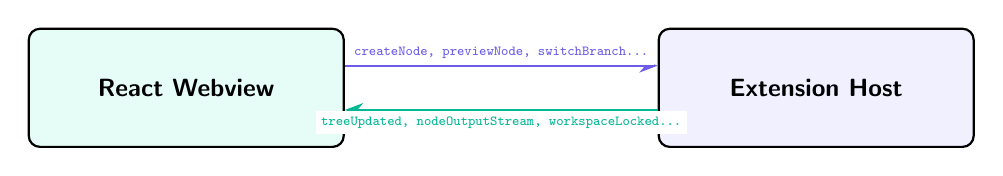
\begin{tikzpicture}[
    box/.style={draw, rounded corners=4pt, thick, minimum width=4cm, minimum height=1.5cm, align=center, font=\small\sffamily},
    msg/.style={font=\tiny\ttfamily, fill=white, inner sep=2pt},
]
    \node[box, fill=nodeGreen!15] (wv) at (0,0) {\textbf{React Webview}};
    \node[box, fill=nodePurple!15] (ext) at (8,0) {\textbf{Extension Host}};

    \draw[-Stealth, thick, zygotePrimary] ([yshift=8pt]wv.east) -- ([yshift=8pt]ext.west)
        node[msg, midway, above] {createNode, previewNode, switchBranch...};
    \draw[-Stealth, thick, zygoteSecondary] ([yshift=-8pt]ext.west) -- ([yshift=-8pt]wv.east)
        node[msg, midway, below] {treeUpdated, nodeOutputStream, workspaceLocked...};
\end{tikzpicture}
\end{center}

\newpage

% ══════════════════════════════════════════════════════════════
\section{Module Deep Dives}
% ══════════════════════════════════════════════════════════════

This section walks through each source file in detail.

% ── 6.1 extension.ts ──
\subsection{Entry Point: extension.ts}

\begin{filebox}{src/extension.ts \quad (68 lines)}
This is where VS Code loads Zygote. It runs once when the extension activates.

\textbf{What it does:}
\begin{enumerate}
    \item Initializes the debug logger
    \item Registers three VS Code commands:
    \begin{itemize}
        \item \texttt{zygote.open} --- loads the tree from disk, creates/shows the webview panel
        \item \texttt{zygote.captureSnapshot} --- saves a debug snapshot
        \item \texttt{zygote.dumpTree} --- dumps the full tree for debugging
    \end{itemize}
\end{enumerate}

\textbf{Activation trigger:} The \texttt{package.json} declares \texttt{onCommand:zygote.open}, so VS Code only loads Zygote when the user first runs that command.
\end{filebox}

% ── 6.2 ZygotePanel.ts ──
\subsection{The Brain: ZygotePanel.ts}

\begin{filebox}{src/webview/ZygotePanel.ts \quad ($\sim$900 lines)}
This is the largest and most important file. It is a \textbf{singleton class} that:

\begin{enumerate}
    \item Creates and manages the VS Code webview panel
    \item Holds the \texttt{ZygoteTree} (the single source of truth)
    \item Routes every message from the webview to the right handler
    \item Orchestrates complex workflows (create node $\to$ run agent $\to$ update tree)
    \item Handles file restoration during branch switches
\end{enumerate}

\textbf{Key instance fields:}
\begin{itemize}
    \item \texttt{tree: ZygoteTree} --- the current tree state
    \item \texttt{activeRunNodeId: NodeId | null} --- tracks which node is currently being previewed
    \item \texttt{pendingCheckoutNodeId: NodeId | null} --- file restore queued for after execution
\end{itemize}

\textbf{Message routing:}
Every message from the webview hits \texttt{handleMessage()}, which dispatches to specific handlers like \texttt{handleCreateNode()}, \texttt{handlePreviewNode()}, \texttt{handleSwitchBranch()}, etc.
\end{filebox}

% ── 6.3 tree.ts ──
\subsection{Pure State Logic: tree.ts}

\begin{filebox}{src/state/tree.ts \quad ($\sim$450 lines)}
This file contains \textbf{pure functions} that operate on the \texttt{ZygoteTree} data structure. No side effects, no I/O, no VS Code API calls. Each function takes a tree, returns a modified tree.

\textbf{Functions:}
\end{filebox}

\begin{table}[H]
\centering
\small
\begin{tabular}{@{}p{4.5cm}p{9cm}@{}}
\toprule
\textbf{Function} & \textbf{What It Does} \\
\midrule
\texttt{createDefaultTree()} & Creates empty tree with a ``main'' branch \\
\texttt{createNode(tree, parentId, prompt)} & Creates a draft node. If parent already has a child on the active branch, \textbf{auto-forks} a new branch \\
\texttt{updateNodePrompt()} & Edits a draft node's prompt (immutable copy) \\
\texttt{updateNodeTitle()} & Renames a node \\
\texttt{setNodeStatus()} & Transitions node state with optional extra data \\
\texttt{appendChatMessage()} & Adds a message to a node's chat array \\
\texttt{deleteNode()} & Removes a leaf-only node (prunes a now-empty forked branch) \\
\texttt{deleteBranch()} & Cascade deletes branch + all descendant nodes \\
\texttt{switchBranch()} & Changes \texttt{activeBranchId} \\
\texttt{rejectPreview()} & Reverts a committed node back to draft \\
\texttt{getBranchNodes()} & Returns the path from root to branch head \\
\texttt{getNodeChildren()} & Returns all children of a node \\
\bottomrule
\end{tabular}
\end{table}

\begin{conceptbox}{Auto-Branching Algorithm}
When \texttt{createNode()} is called with a parent that already has a child on the active branch:

\begin{lstlisting}
// Pseudocode
if (parent already has child on active branch) {
    // Auto-fork: create new branch
    newBranch = { parentBranchId: activeBranch, forkedAtNodeId: parentId }
    // New node goes on the new branch
}
\end{lstlisting}

\textbf{Why?} This prevents accidentally creating a linear chain when the user wants to try an alternative. If you're at Node 2 and it already has a child (Node 3) on the current branch, creating another child automatically forks into a new branch.
\end{conceptbox}

% ── 6.4 persistence.ts ──
\subsection{Disk I/O: persistence.ts}

\begin{filebox}{src/state/persistence.ts \quad (90 lines)}
Simple file I/O for the tree state:

\begin{itemize}
    \item \texttt{loadTree(workspaceRoot)} --- reads \texttt{.zygote/tree.json}. If missing, returns a fresh default tree. Includes recovery logic: fixes orphaned nodes, resets nodes stuck in ``previewing'' status.
    \item \texttt{saveTree(workspaceRoot, tree)} --- writes tree as JSON to \texttt{.zygote/tree.json}. Auto-creates the \texttt{.zygote/} directory.
    \item \texttt{ensureZygoteDir(workspaceRoot)} --- ensures \texttt{.zygote/snapshots/} exists.
\end{itemize}
\end{filebox}

% ── 6.5 snapshots.ts ──
\subsection{File Versioning: snapshots.ts}

\begin{filebox}{src/state/snapshots.ts \quad (107 lines)}
Content-addressable file storage, like a mini-Git object store.
\end{filebox}

\begin{center}
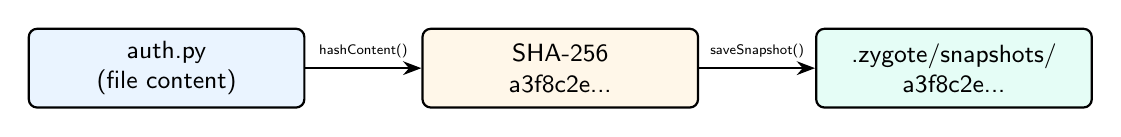
\begin{tikzpicture}[
    box/.style={draw, rounded corners=3pt, thick, minimum width=3.5cm, minimum height=1cm, align=center, font=\small\sffamily},
    arrow/.style={-Stealth, thick},
]
    \node[box, fill=nodeBlue!15] (file) at (0, 0) {auth.py\\(file content)};
    \node[box, fill=nodeOrange!15] (hash) at (5, 0) {SHA-256\\a3f8c2e...};
    \node[box, fill=nodeGreen!15] (store) at (10, 0) {.zygote/snapshots/\\a3f8c2e...};

    \draw[arrow] (file) -- (hash) node[above, midway, font=\tiny\sffamily] {hashContent()};
    \draw[arrow] (hash) -- (store) node[above, midway, font=\tiny\sffamily] {saveSnapshot()};
\end{tikzpicture}
\end{center}

\textbf{Key functions:}
\begin{itemize}
    \item \texttt{hashContent(content)} --- SHA-256 hash of file content
    \item \texttt{saveSnapshot(workspaceRoot, content)} --- Store blob under its hash. Skip if already exists (dedup).
    \item \texttt{loadSnapshot(workspaceRoot, hash)} --- Retrieve stored content by hash.
    \item \texttt{captureWorkspaceSnapshot(root, paths)} --- Hash multiple files at once.
    \item \texttt{restoreWorkspaceSnapshot(root, fileHashes)} --- Restore all files from their hashes.
\end{itemize}

\begin{keypoint}
\textbf{Deduplication:} If two nodes have the same version of a file, they share the same snapshot blob. Storage is proportional to the number of \textit{unique} file contents, not the number of nodes.
\end{keypoint}

% ── 6.6 claude.ts ──
\subsection{API Client: claude.ts}

\begin{filebox}{src/agent/claude.ts \quad (84 lines)}
Singleton wrapper around the Anthropic SDK:

\begin{itemize}
    \item \texttt{getClient(secretStorage)} --- Creates or returns the cached Anthropic client. Reads API key from VS Code's secret storage or the \texttt{ANTHROPIC\_API\_KEY} environment variable.
    \item \texttt{resetClient()} --- Clears the cached client (e.g., after API key change).
    \item \texttt{sendMessage(client, options)} --- Calls the Claude API with streaming enabled.
    \item Model used: \texttt{claude-sonnet-4-20250514}
\end{itemize}
\end{filebox}

% ── 6.7 tools.ts ──
\subsection{Agent Tools: tools.ts}

\begin{filebox}{src/agent/tools.ts \quad (192 lines)}
Defines the 4 tools that Claude can use during execution:
\end{filebox}

\begin{table}[H]
\centering
\begin{tabular}{@{}p{3cm}p{3.5cm}p{6.5cm}@{}}
\toprule
\textbf{Tool} & \textbf{Parameters} & \textbf{Behavior} \\
\midrule
\texttt{read\_file} & path (relative) & Reads file content from workspace \\
\texttt{list\_files} & path (relative) & Lists directory contents. Filters out \texttt{.zygote/}, \texttt{node\_modules} \\
\texttt{write\_file} & path, content & Writes or creates a file. Auto-creates parent directories \\
\texttt{search\_files} & pattern (regex) & Regex search across all workspace files. Max 50 matches \\
\bottomrule
\end{tabular}
\end{table}

\texttt{executeTool(workspaceRoot, toolName, input)} dispatches a tool call to the right handler and returns the result.

% ── 6.8 runner.ts ──
\subsection{Agent Execution: runner.ts}

\begin{filebox}{src/agent/runner.ts \quad ($\sim$450 lines)}
This is where the AI actually runs. It manages the full lifecycle of a preview.
\end{filebox}

\subsubsection{The runPreview() Workflow}

\begin{center}
\begin{tikzpicture}[
    step/.style={draw, rounded corners=4pt, thick, minimum width=4cm, minimum height=0.8cm, align=center, font=\small\sffamily, fill=codeBg},
    arrow/.style={-Stealth, thick, zygotePrimary},
    note/.style={font=\tiny\sffamily\color{gray}, align=left},
]
    \node[step] (s1) at (0, 0) {1. Set status = ``previewing''};
    \node[step] (s2) at (0, -1.3) {2. Capture pre-snapshot};
    \node[step] (s3) at (0, -2.6) {3. Build context from ancestors};
    \node[step] (s4) at (0, -3.9) {4. Call Claude API (streaming)};
    \node[step] (s5) at (0, -5.2) {5. Execute tool calls};
    \node[step] (s6) at (0, -6.5) {6. Stream text to webview};
    \node[step] (s7) at (0, -7.8) {7. Capture post-snapshot};
    \node[step] (s8) at (0, -9.1) {8. Set status = ``committed''};
    \node[step] (s9) at (0, -10.4) {9. Save tree to disk};

    \foreach \i [evaluate=\i as \j using int(\i+1)] in {1,...,8} {
        \draw[arrow] (s\i) -- (s\j);
    }

    \node[note, right=0.5cm of s2] {Hash ALL workspace files\\before agent touches anything};
    \node[note, right=0.5cm of s3] {Concatenate ancestor nodes'\\prompt + response pairs};
    \node[note, right=0.5cm of s4] {SDK backend or CLI backend\\(configurable)};
    \node[note, right=0.5cm of s5] {read\_file, write\_file, etc.\\Results sent back to Claude};
    \node[note, right=0.5cm of s7] {Hash all files AFTER agent\\to record what changed};
\end{tikzpicture}
\end{center}

\subsubsection{Context Construction}

When the agent runs, it needs to know about prior work. The context is built by walking up the ancestor chain:

\begin{lstlisting}
// Pseudocode for context building
ancestors = walkUp(node.parentId) // get all ancestors in order
context = ancestors.map(n =>
    `User: ${n.prompt}\nAssistant: ${n.agentResponse}`
).join("\n\n---\n\n")

// Plus the current node's chat messages
context += node.chat.map(m =>
    `${m.role}: ${m.content}`
).join("\n\n")
\end{lstlisting}

This means the agent always sees the full decision history leading to the current node.

\subsubsection{Two Backend Implementations}

\begin{table}[H]
\centering
\begin{tabular}{@{}p{2.5cm}p{5cm}p{5.5cm}@{}}
\toprule
\textbf{Backend} & \textbf{How It Works} & \textbf{When Used} \\
\midrule
\textbf{SDK} & Direct API calls via \texttt{@anthropic-ai/sdk} & When API key is available \\
\textbf{CLI} & Spawns \texttt{claude --print --output-format stream-json} as child process & Fallback when SDK unavailable \\
\bottomrule
\end{tabular}
\end{table}

\texttt{resolveBackend()} checks for an SDK API key first, falls back to CLI.

\newpage

% ══════════════════════════════════════════════════════════════
\section{The React UI}
% ══════════════════════════════════════════════════════════════

The webview is a React app built with Vite, running inside a VS Code webview sandbox.

\subsection{UI Layout}

\begin{center}
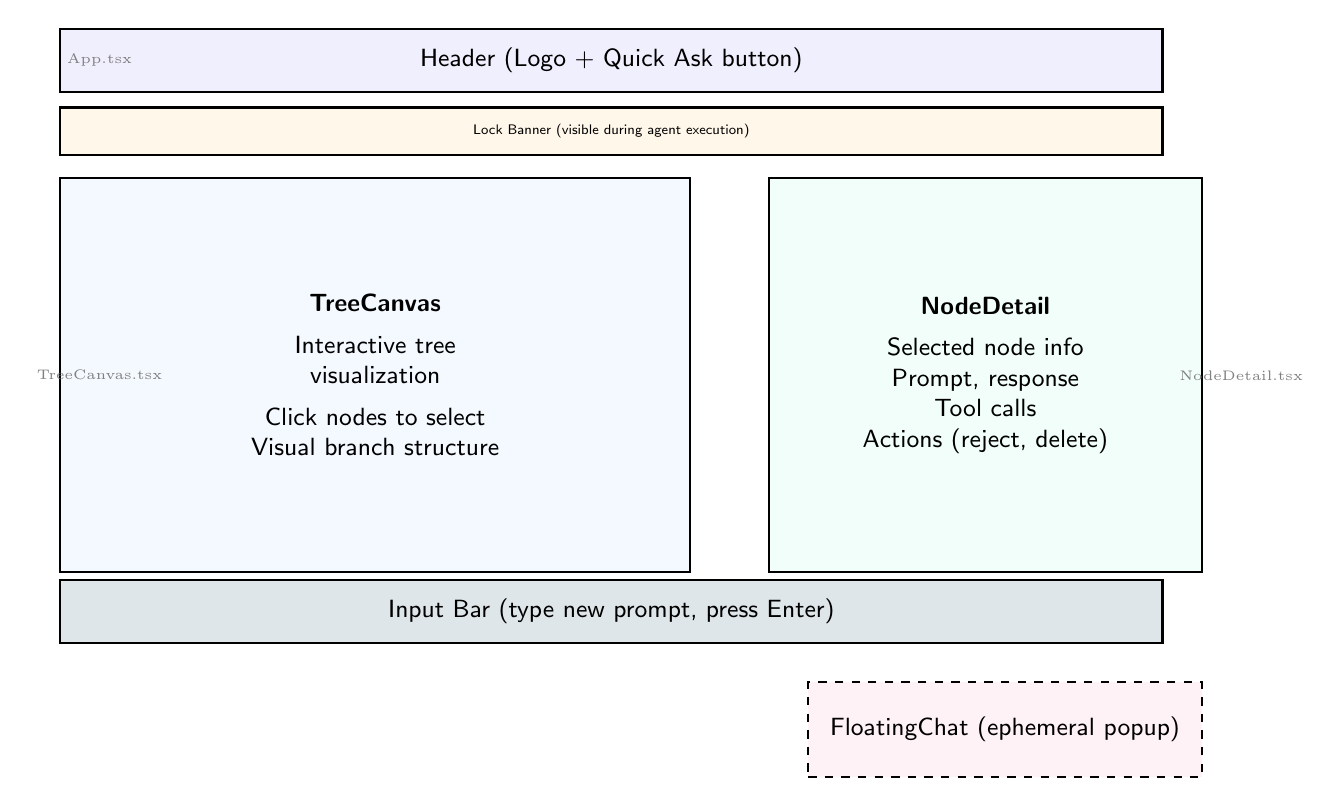
\begin{tikzpicture}[
    region/.style={draw, thick, minimum height=1cm, align=center, font=\small\sffamily},
]
    % Header
    \node[region, fill=zygotePrimary!10, minimum width=14cm, minimum height=0.8cm] (header) at (0, 5) {Header (Logo + Quick Ask button)};

    % Lock banner
    \node[region, fill=nodeOrange!15, minimum width=14cm, minimum height=0.6cm] (lock) at (0, 4.1) {\tiny Lock Banner (visible during agent execution)};

    % Main body
    \node[region, fill=nodeBlue!8, minimum width=8cm, minimum height=5cm] (canvas) at (-3, 1) {
        \textbf{TreeCanvas}\\[4pt]
        Interactive tree\\
        visualization\\[4pt]
        Click nodes to select\\
        Visual branch structure
    };
    \node[region, fill=nodeGreen!8, minimum width=5.5cm, minimum height=5cm] (detail) at (4.75, 1) {
        \textbf{NodeDetail}\\[4pt]
        Selected node info\\
        Prompt, response\\
        Tool calls\\
        Actions (reject, delete)
    };

    % Input bar
    \node[region, fill=zygoteLight, minimum width=14cm, minimum height=0.8cm] (input) at (0, -2) {Input Bar (type new prompt, press Enter)};

    % Floating chat
    \node[region, fill=zygoteAccent!10, minimum width=5cm, minimum height=1.2cm, dashed] (float) at (5, -3.5) {FloatingChat (ephemeral popup)};

    % Labels
    \node[font=\tiny\color{gray}] at (-6.5, 5) {App.tsx};
    \node[font=\tiny\color{gray}] at (-6.5, 1) {TreeCanvas.tsx};
    \node[font=\tiny\color{gray}] at (8, 1) {NodeDetail.tsx};
\end{tikzpicture}
\end{center}

\subsection{Component Breakdown}

\begin{table}[H]
\centering
\small
\begin{tabular}{@{}p{4cm}p{9.5cm}@{}}
\toprule
\textbf{Component} & \textbf{Responsibility} \\
\midrule
\texttt{App.tsx} (470 lines) & Root component. Manages all state: tree, selected node, streaming text, workspace lock, error messages. Renders layout. \\
\texttt{TreeCanvas.tsx} & Renders the tree as an interactive canvas/SVG. Nodes connected with lines. Click to select. \\
\texttt{NodeDetail.tsx} & Right panel. Shows prompt, agent response (markdown), thinking blocks, tool calls, action buttons. \\
\texttt{NodeChat.tsx} & Chat interface within a draft node for pre-execution conversation. \\
\texttt{FloatingChat.tsx} & Ephemeral quick-ask dialog. Not persisted to tree. \\
\texttt{BranchSelector.tsx} & Dropdown to switch between branches. \\
\texttt{MarkdownRenderer.tsx} & Renders agent output using \texttt{react-markdown} + syntax highlighting. \\
\texttt{ThinkingBlock.tsx} & Expandable/collapsible display of Claude's thinking blocks. \\
\bottomrule
\end{tabular}
\end{table}

\subsection{Key State in App.tsx}

\begin{lstlisting}
// Core state variables in App.tsx
const [tree, setTree] = useState<ZygoteTree | null>(null);
const [selectedNodeId, setSelectedNodeId] = useState<NodeId | null>(null);
const [streamingText, setStreamingText] = useState<Record<NodeId, string>>({});
const [thinkingText, setThinkingText] = useState<Record<NodeId, string>>({});
const [workspaceLock, setWorkspaceLock] = useState<{nodeId, title} | null>(null);
const [errorMessage, setErrorMessage] = useState<string | null>(null);
const [inputValue, setInputValue] = useState<string>("");
\end{lstlisting}

\newpage

% ══════════════════════════════════════════════════════════════
\section{Complete Data Flow Walkthroughs}
% ══════════════════════════════════════════════════════════════

These walkthroughs trace exactly what happens for each major user action, from click to result.

\subsection{Walkthrough 1: Creating a Node and Running the Agent}

\begin{enumerate}[label=\textbf{Step \arabic*:}, leftmargin=3cm]
    \item \textbf{User types ``refactor auth.py'' and presses Enter}
    \begin{itemize}
        \item \texttt{App.tsx} calls \texttt{postMessage(\{ type: `createNode', parentId: null, prompt: `refactor auth.py' \})}
    \end{itemize}

    \item \textbf{Extension receives message}
    \begin{itemize}
        \item \texttt{ZygotePanel.handleMessage()} routes to \texttt{handleCreateNode()}
        \item Calls \texttt{createNode(tree, null, `refactor auth.py')} from \texttt{tree.ts}
        \item New draft node created with UUID, added to \texttt{tree.nodes}
        \item \texttt{tree.rootNodeIds} updated (since parentId is null)
        \item Branch head updated to point to new node
    \end{itemize}

    \item \textbf{Auto-summarize title (non-blocking)}
    \begin{itemize}
        \item Calls \texttt{handleQuickAsk(`Summarize as 3-5 word title: refactor auth.py')}
        \item Updates \texttt{node.title} when response arrives
        \item Sends \texttt{treeUpdated} to webview
    \end{itemize}

    \item \textbf{Immediately starts preview execution}
    \begin{itemize}
        \item Sends \texttt{workspaceLocked \{ nodeId, title \}} to webview
        \item Calls \texttt{runPreview(tree, nodeId, secretStorage, callbacks)}
    \end{itemize}

    \item \textbf{Inside runPreview():}
    \begin{itemize}
        \item Sets node status to ``previewing''
        \item \texttt{captureWorkspaceSnapshot()} --- hashes ALL workspace files (pre-snapshot)
        \item Builds context: since this is a root node, context is just the prompt
        \item Calls Claude API with the 4 tool definitions
        \item \textbf{Streaming loop:} For each chunk from Claude:
        \begin{itemize}
            \item Text $\to$ sends \texttt{nodeOutputStream \{ nodeId, delta \}} to webview
            \item Thinking $\to$ sends \texttt{nodeThinkingStream \{ nodeId, delta \}} to webview
            \item Tool call $\to$ executes via \texttt{executeTool()}, sends result back to Claude
        \end{itemize}
        \item After Claude finishes: \texttt{captureWorkspaceSnapshot()} again (post-snapshot)
        \item Sets node status to ``committed'' with agentResponse, toolCalls, workspaceSnapshot
        \item \texttt{saveTree()} writes to disk
    \end{itemize}

    \item \textbf{Webview receives updates}
    \begin{itemize}
        \item \texttt{nodeOutputStream} $\to$ accumulates in \texttt{streamingText[nodeId]}
        \item \texttt{treeUpdated} $\to$ replaces full tree state
        \item Node in TreeCanvas shows ``committed'' status with green indicator
        \item NodeDetail shows rendered markdown response + tool calls
    \end{itemize}
\end{enumerate}

\subsection{Walkthrough 2: Auto-Forking a Branch}

\textit{Note: branching is implicit. There is no explicit ``Fork'' action or \texttt{forkNode()} function --- a new branch is created automatically by \texttt{createNode()} whenever a second child is added to a node that already has a child on the active branch.}

\begin{enumerate}[label=\textbf{Step \arabic*:}, leftmargin=3cm]
    \item \textbf{User adds a second continuation from a node}
    \begin{itemize}
        \item With node \texttt{abc123} selected --- a node that \textit{already} has a child on the active branch --- the user types a new prompt and submits
        \item Webview sends \texttt{\{ type: `createNode', parentId: `abc123', prompt: `...' \}}
    \end{itemize}

    \item \textbf{Extension auto-forks}
    \begin{itemize}
        \item Calls \texttt{createNode(tree, `abc123', prompt)} from \texttt{tree.ts}
        \item Detects that \texttt{abc123} already has a child on the active branch, so it forks a new \texttt{ZygoteBranch}: \texttt{\{ name: `branch-N', parentBranchId, forkedAtNodeId: `abc123' \}}
        \item Branch creation is O(1) --- no nodes are copied. The new draft node is placed on the new branch, which becomes active
    \end{itemize}

    \item \textbf{Preview run}
    \begin{itemize}
        \item The extension immediately runs the new node via \texttt{runPreview()}: capture ``before'' snapshot $\to$ agent executes $\to$ capture ``after'' snapshot $\to$ commit
        \item \texttt{saveTree()} persists; \texttt{treeUpdated} is sent to the webview
    \end{itemize}

    \item \textbf{Webview updates}
    \begin{itemize}
        \item TreeCanvas shows the new branch as a parallel line forking from \texttt{abc123}
        \item Selecting any node auto-switches \texttt{activeBranchId} to that node's branch (no manual branch picker needed)
    \end{itemize}
\end{enumerate}

\subsection{Walkthrough 3: Rejecting a Preview}

\begin{enumerate}[label=\textbf{Step \arabic*:}, leftmargin=3cm]
    \item \textbf{User clicks ``Reject'' on a committed node}
    \begin{itemize}
        \item Webview sends \texttt{\{ type: `rejectPreview', nodeId \}}
    \end{itemize}

    \item \textbf{Extension reverts}
    \begin{itemize}
        \item Calls \texttt{rejectPreview(tree, nodeId)} from \texttt{tree.ts}
        \item Sets node status back to ``draft''
        \item Clears agentResponse, toolCalls, workspaceSnapshot
        \item Restores files from the \textit{pre-snapshot} (the state before the agent ran)
    \end{itemize}

    \item \textbf{User can now edit the prompt and try again}
    \begin{itemize}
        \item Node is back in draft state
        \item Files are back to their pre-execution state
        \item Full preview--reject--edit--preview loop is possible
    \end{itemize}
\end{enumerate}

\subsection{Walkthrough 4: Switching Branches}

\begin{enumerate}[label=\textbf{Step \arabic*:}, leftmargin=3cm]
    \item \textbf{User selects a different branch from BranchSelector}
    \begin{itemize}
        \item Webview sends \texttt{\{ type: `switchBranch', branchId \}}
    \end{itemize}

    \item \textbf{Extension switches}
    \begin{itemize}
        \item \texttt{switchBranch(tree, branchId)} sets \texttt{activeBranchId}
        \item Finds the head node of the target branch
        \item Restores files from head node's \texttt{workspaceSnapshot.fileHashes}
        \item Your editor now shows the files as they were on that branch
    \end{itemize}

    \item \textbf{Webview re-renders}
    \begin{itemize}
        \item TreeCanvas highlights the active branch
        \item NodeDetail updates to show the head node
    \end{itemize}
\end{enumerate}

\newpage

% ══════════════════════════════════════════════════════════════
\section{File Snapshot System (Deep Dive)}
% ══════════════════════════════════════════════════════════════

The snapshot system is how Zygote guarantees that switching branches or rejecting previews always restores the exact file state. It works like Git's object store.

\subsection{How It Works}

\begin{center}
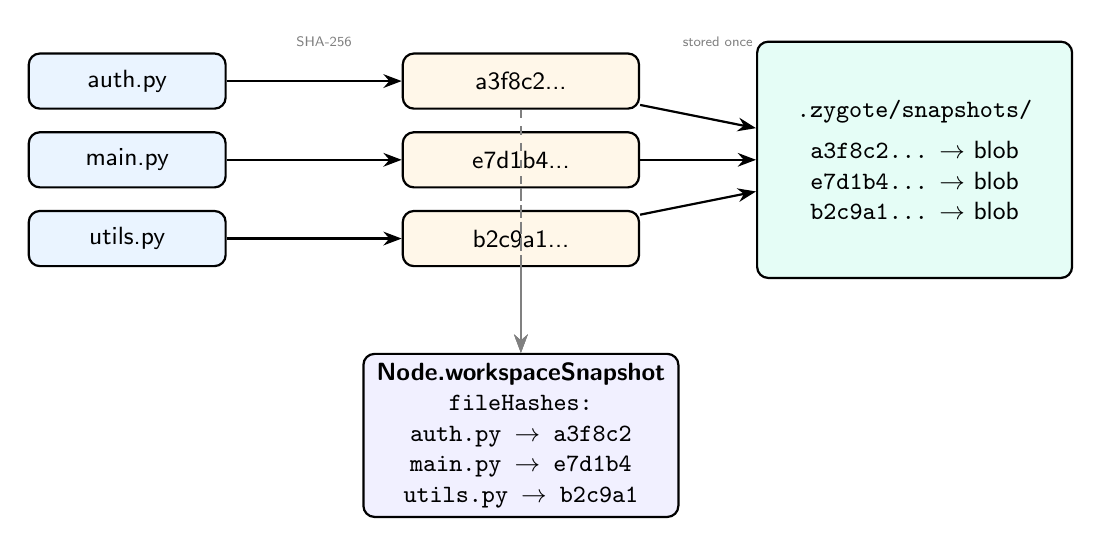
\begin{tikzpicture}[
    box/.style={draw, rounded corners=4pt, thick, align=center, font=\small\sffamily},
    arrow/.style={-Stealth, thick},
]
    % Files
    \node[box, fill=nodeBlue!15, minimum width=2.5cm, minimum height=0.7cm] (f1) at (0, 2) {auth.py};
    \node[box, fill=nodeBlue!15, minimum width=2.5cm, minimum height=0.7cm] (f2) at (0, 1) {main.py};
    \node[box, fill=nodeBlue!15, minimum width=2.5cm, minimum height=0.7cm] (f3) at (0, 0) {utils.py};

    % Hashes
    \node[box, fill=nodeOrange!15, minimum width=3cm, minimum height=0.7cm] (h1) at (5, 2) {a3f8c2...};
    \node[box, fill=nodeOrange!15, minimum width=3cm, minimum height=0.7cm] (h2) at (5, 1) {e7d1b4...};
    \node[box, fill=nodeOrange!15, minimum width=3cm, minimum height=0.7cm] (h3) at (5, 0) {b2c9a1...};

    % Snapshot store
    \node[box, fill=nodeGreen!15, minimum width=4cm, minimum height=3cm] (store) at (10, 1) {
        \texttt{.zygote/snapshots/}\\[4pt]
        \texttt{a3f8c2...} $\to$ blob\\
        \texttt{e7d1b4...} $\to$ blob\\
        \texttt{b2c9a1...} $\to$ blob
    };

    % Node
    \node[box, fill=nodePurple!15, minimum width=4cm, minimum height=2cm] (node) at (5, -2.5) {
        \textbf{Node.workspaceSnapshot}\\
        \texttt{fileHashes:}\\
        \texttt{auth.py $\to$ a3f8c2}\\
        \texttt{main.py $\to$ e7d1b4}\\
        \texttt{utils.py $\to$ b2c9a1}
    };

    \draw[arrow] (f1) -- (h1);
    \draw[arrow] (f2) -- (h2);
    \draw[arrow] (f3) -- (h3);
    \draw[arrow] (h1) -- (store);
    \draw[arrow] (h2) -- (store);
    \draw[arrow] (h3) -- (store);
    \draw[arrow, dashed, gray] (h1) -- (node);
    \draw[arrow, dashed, gray] (h2) -- (node);
    \draw[arrow, dashed, gray] (h3) -- (node);

    \node[font=\tiny\sffamily\color{gray}] at (2.5, 2.5) {SHA-256};
    \node[font=\tiny\sffamily\color{gray}] at (7.5, 2.5) {stored once};
\end{tikzpicture}
\end{center}

\subsection{Deduplication Example}

\begin{center}
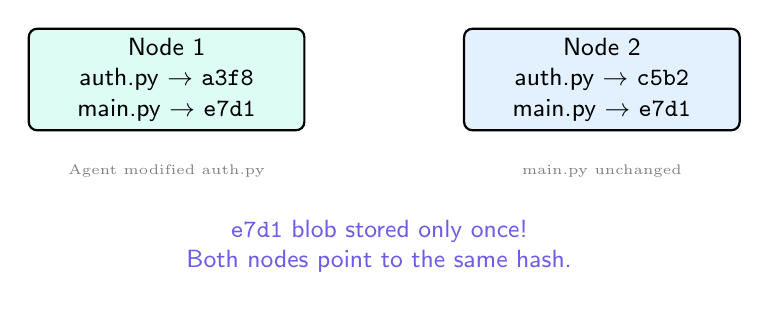
\begin{tikzpicture}[
    node distance=0.8cm,
    box/.style={draw, rounded corners=3pt, thick, minimum width=3.5cm, minimum height=1.2cm, align=center, font=\small\sffamily},
]
    \node[box, fill=nodeGreen!20] (n1) {Node 1\\auth.py $\to$ \texttt{a3f8}\\main.py $\to$ \texttt{e7d1}};
    \node[box, fill=nodeBlue!20, right=2cm of n1] (n2) {Node 2\\auth.py $\to$ \texttt{c5b2}\\main.py $\to$ \texttt{e7d1}};

    \node[draw=none, below=0.3cm of n1, font=\tiny\color{gray}] {Agent modified auth.py};
    \node[draw=none, below=0.3cm of n2, font=\tiny\color{gray}] {main.py unchanged};
    \node[draw=none, below=1cm of n1, font=\small\sffamily, text=zygotePrimary, align=center, xshift=2.7cm] {
        \texttt{e7d1} blob stored only once!\\
        Both nodes point to the same hash.
    };
\end{tikzpicture}
\end{center}

\newpage

% ══════════════════════════════════════════════════════════════
\section{Persistence Format}
% ══════════════════════════════════════════════════════════════

All state is stored in \texttt{.zygote/tree.json}. Here is an annotated example:

\begin{lstlisting}
{
  "workspaceRoot": "/path/to/workspace",
  "activeBranchId": "branch-main-uuid",
  "rootNodeIds": ["node-1-uuid"],

  "nodes": {
    "node-1-uuid": {
      "id": "node-1-uuid",
      "parentId": null,
      "branchId": "branch-main-uuid",
      "status": "committed",
      "title": "Refactor auth module",
      "prompt": "Refactor the authentication...",
      "chat": [
        { "role": "user", "content": "...", "timestamp": 1234567890 }
      ],
      "agentResponse": "I'll refactor the auth module...",
      "toolCalls": [
        {
          "tool": "read_file",
          "input": { "path": "auth.py" },
          "result": { "ok": true, "data": "..." }
        }
      ],
      "workspaceSnapshot": {
        "fileHashes": {
          "auth.py": "a3f8c2e...",
          "main.py": "e7d1b4f..."
        }
      },
      "tokens": { "input": 500, "output": 800 }
    }
  },

  "branches": {
    "branch-main-uuid": {
      "id": "branch-main-uuid",
      "name": "main",
      "headNodeId": "node-1-uuid",
      "createdAt": 1234567890
    }
  }
}
\end{lstlisting}

\newpage

% ══════════════════════════════════════════════════════════════
\section{Debug System}
% ══════════════════════════════════════════════════════════════

\begin{filebox}{src/debug/logger.ts \quad (317 lines)}
The \texttt{DebugLogger} class writes structured logs to \texttt{.debug/session.jsonl} for diagnosing issues.

\textbf{Log methods:}
\begin{itemize}
    \item \texttt{info(category, message, data?)} --- informational
    \item \texttt{warn(category, message, data?)} --- warnings
    \item \texttt{error(category, message, data?)} --- errors
\end{itemize}

\textbf{Diagnostic methods:}
\begin{itemize}
    \item \texttt{captureSnapshot(tree, extra)} --- saves a full error analysis to \texttt{.debug/snapshot.json}
    \item \texttt{dumpTree(tree, extra)} --- writes a human-readable markdown dump to \texttt{.debug/tree-dump.md} including:
    \begin{itemize}
        \item Branch summary (name, head, parent)
        \item Full node hierarchy (indented)
        \item Status icons, token counts, errors
        \item Chat history per node
        \item Tool call details
        \item Full context chain (what was sent to the agent)
    \end{itemize}
\end{itemize}

\textbf{Log rotation:} Files rotate at 2MB to prevent unbounded growth.
\end{filebox}

\newpage

% ══════════════════════════════════════════════════════════════
\section{Build and Run}
% ══════════════════════════════════════════════════════════════

\subsection{Build Scripts}

\begin{table}[H]
\centering
\begin{tabular}{@{}p{4.5cm}p{9cm}@{}}
\toprule
\textbf{Script} & \textbf{What It Does} \\
\midrule
\texttt{npm run compile} & Compiles extension TypeScript $\to$ \texttt{dist/} \\
\texttt{npm run build:webview} & Builds React UI with Vite $\to$ \texttt{webview-ui/dist/} \\
\texttt{npm run build} & Both of the above \\
\texttt{npm run package} & Creates \texttt{.vsix} file for distribution \\
\bottomrule
\end{tabular}
\end{table}

\subsection{Development Workflow}

\begin{enumerate}
    \item Open the Zygote repo in VS Code
    \item Press \texttt{F5} to launch the Extension Development Host
    \item In the new VS Code window, run command \texttt{Zygote: Open}
    \item The Zygote webview panel opens on the right
    \item Make changes to \texttt{src/} $\to$ recompile $\to$ restart Extension Host
    \item Make changes to \texttt{webview-ui/} $\to$ rebuild webview $\to$ reload webview
\end{enumerate}

\subsection{Extension Manifest (package.json)}

Key configuration:
\begin{itemize}
    \item \texttt{main: "dist/extension.js"} --- compiled entry point
    \item \texttt{engines.vscode: "\^{}1.100.0"} --- minimum VS Code version
    \item \texttt{activationEvents: ["onCommand:zygote.open"]} --- lazy activation
    \item \texttt{contributes.commands} --- registers 3 commands
    \item \texttt{contributes.configuration.zygote.backend} --- setting: ``auto'' | ``sdk'' | ``cli''
\end{itemize}

\newpage

% ══════════════════════════════════════════════════════════════
\section{What's NOT Built Yet (v0.1 Scope)}
% ══════════════════════════════════════════════════════════════

Understanding what Zygote \textit{doesn't} do is just as important as what it does:

\begin{table}[H]
\centering
\begin{tabular}{@{}p{4.5cm}p{9cm}@{}}
\toprule
\textbf{Missing Feature} & \textbf{Why It Matters} \\
\midrule
Branch merge & You can fork and switch, but not combine two branches \\
Shell/terminal execution & Agent can only read/write files, not run commands \\
Multi-turn agent loops & Each preview is a single agent turn (no iterative fix loops) \\
Side-by-side branch diff & No visual comparison of what changed between branches \\
Settings UI & Configuration is hard-coded \\
Cost tracking & No token usage dashboard or budget controls \\
Multi-user collaboration & Single-user only \\
Large workspace optimization & Designed for small-to-medium projects \\
Rejected preview history & Rejected previews are discarded (not saved for review) \\
\bottomrule
\end{tabular}
\end{table}

\newpage

% ══════════════════════════════════════════════════════════════
\section{Key Design Decisions Summary}
% ══════════════════════════════════════════════════════════════

\begin{table}[H]
\centering
\begin{tabular}{@{}p{4cm}p{5cm}p{4.5cm}@{}}
\toprule
\textbf{Decision} & \textbf{Rationale} & \textbf{Trade-off} \\
\midrule
Flat node map & O(1) lookup, easy JSON serialization & Must traverse parentId for tree ops \\[6pt]
Content-addressable snapshots & Dedup unchanged files across nodes & Must hash every file on capture \\[6pt]
Extension host = source of truth & Webview sandbox can't do I/O & All state flows through one process \\[6pt]
Auto-branching & Prevents accidental linear chains & May create unexpected branches \\[6pt]
Two agent backends & Flexibility (SDK + CLI) & More code to maintain \\[6pt]
Full tree sent on every update & Simple protocol, no partial diffs & Could be slow for very large trees \\[6pt]
Immutable state ops & Predictable, testable, no side effects & Lots of object spreading \\
\bottomrule
\end{tabular}
\end{table}

\newpage

% ══════════════════════════════════════════════════════════════
\section{Quick Reference: File $\to$ Purpose Lookup}
% ══════════════════════════════════════════════════════════════

Use this table as a quick reference when navigating the codebase.

\begin{longtable}{@{}p{6cm}p{7.5cm}@{}}
\toprule
\textbf{File} & \textbf{One-Line Purpose} \\
\midrule
\endhead
\texttt{src/extension.ts} & Extension entry point, registers commands \\
\texttt{src/webview/ZygotePanel.ts} & Message routing hub, state orchestrator \\
\texttt{src/webview/html.ts} & HTML template for webview \\
\texttt{src/state/tree.ts} & Pure tree state operations \\
\texttt{src/state/persistence.ts} & Load/save tree.json \\
\texttt{src/state/snapshots.ts} & Content-addressable file versioning \\
\texttt{src/agent/claude.ts} & Anthropic API client \\
\texttt{src/agent/tools.ts} & 4 tool definitions for the agent \\
\texttt{src/agent/runner.ts} & Agent execution + preview workflow \\
\texttt{src/debug/logger.ts} & Debug logging + tree dumps \\
\texttt{src/shared/types.ts} & TypeScript types for extension $\leftrightarrow$ webview \\
\texttt{webview-ui/src/App.tsx} & Main React component + all UI state \\
\texttt{webview-ui/src/vscode-api.ts} & VS Code API wrapper for webview \\
\texttt{webview-ui/.../TreeCanvas.tsx} & Interactive tree visualization \\
\texttt{webview-ui/.../NodeDetail.tsx} & Right panel node details \\
\texttt{webview-ui/.../NodeChat.tsx} & Chat interface in draft nodes \\
\texttt{webview-ui/.../FloatingChat.tsx} & Quick-ask ephemeral popup \\
\texttt{webview-ui/.../BranchSelector.tsx} & Branch switching dropdown \\
\texttt{webview-ui/.../MarkdownRenderer.tsx} & Markdown + syntax highlighting \\
\texttt{webview-ui/.../ThinkingBlock.tsx} & Expandable thinking blocks \\
\texttt{.zygote/tree.json} & Persisted tree state (runtime) \\
\texttt{.zygote/snapshots/*} & File content blobs (runtime) \\
\texttt{package.json} & Extension manifest + dependencies \\
\texttt{SPEC.md} & Product specification \\
\bottomrule
\end{longtable}

\vfill

\begin{center}
\textcolor{gray}{\rule{6cm}{0.4pt}}\\[0.5cm]
{\large\textcolor{zygotePrimary}{End of Zygote Architecture Guide}}\\[0.3cm]
{\small\textcolor{gray}{Read each section in order, or jump to any section by topic.\\
Use this document alongside the codebase to build your understanding.}}
\end{center}

\end{document}
